\documentclass{article}

\usepackage{graphicx}
\usepackage{indentfirst}
\usepackage{booktabs}
\usepackage[a4paper, total={6in, 8in}]{geometry}
\usepackage{hyperref}
\usepackage{fancyhdr}
\usepackage{subcaption}
\usepackage{xepersian}
\usepackage{fontspec}
\usepackage{url}
\settextfont[Scale=1.2,ExternalLocation=fonts/,BoldFont=B Nazanin Bold.ttf]{B Nazanin}
\setlatintextfont[Scale=1.2,ExternalLocation=fonts/,BoldFont=XB Zar.ttf]{Times New Roman}

\begin{document}


%title page%
\begin{titlepage}
	\begin{center}
		\vspace{0.2cm}
		
		
\includegraphics[width=0.4\textwidth]{sharif.png}\\
		\vspace{0.5cm}
		\textbf{ \Huge{فاز دوم}}\\
		\vspace{0.25cm}
		\textbf{ \Large{پروژه مقدمه‌ای بر بیوانفورماتیک \\ دکتر علی  شریفی‌زارچی و دکتر سمیه کوهی}}
		\vspace{0.2cm}
		
		
		\large \textbf{دانشکده مهندسی کامپیوتر}\\\vspace{0.1cm}
		\large   دانشگاه صنعتی شریف\\\vspace{0.2cm}
		\large   ﻧﯿﻢ‌سال اول ۰۱-۰۲ \\\vspace{0.2cm}
		\large{\Large{امیرحسین باقری - 98105621}}\\
		\large{\Large{مهدی مستانی - 97100513}}\\
		\large{\Large{محمدرضا مفیضی - 98106059}}\\
	\end{center}
\end{titlepage}
%title page%

\newpage
\tableofcontents
\newpage
%pages header
\pagestyle{fancy}
\fancyhf{}
\fancyfoot{}
\setlength{\headheight}{59pt}
\cfoot{\thepage}
\lhead{فاز دوم}
\rhead{
\includegraphics[width=0.1\textwidth]{sharif.png}\\
		دانشکده مهندسی کامپیوتر
}
\chead{پروژه مقدمه‌ای بر بیوانفورماتیک}
%pages header

\section{بیان ژن‌ها}
\subsection{انتخاب تمام نمونه‌های سالم}
در جدول \ref{tab:genes} ژن‌هایی که بیان آن‌ها به طرز معناداری بین گروه سالم و گروه بیماران متفاوت است را نمایش می‌دهیم
\footnote{جدول کامل به همراه این گزارش ضمیمه شده است.}.

\begin{table}[h!]
	\begin{latin}
		\begin{center}
			\begin{tabular}{@{}cccc@{}}
				\toprule
				Gene Symbol & Gene ID & Adj. P-Val & logFC  \\ \midrule
				MPO         & 4353    & 3.617e-19 & -5.563 \\
				FLT3        & 2322    & 4.835e-19 & -5.250 \\
				KIAA0101    & 9768    & 6.308e-19 & -4.559 \\
				BUB1B       & 701     & 1.664e-18 & -2.756 \\
				SUCNR1      & 56670   & 1.938e-18 & -2.996 \\ \bottomrule
			\end{tabular}
		\end{center}
	\end{latin}
	\caption{5 ژنی که بیان آن‌ها به طرز معناداری بین گروه سالم و گروه بیماران متفاوت است.}
	\label{tab:genes}
\end{table}

حالا ژن‌هایی که در بیماران از بقیه بیشتر بیان شده‌اند و همچنین ژن‌هایی که کمتر از بقیه بیان شده‌اند را در جدول \ref{tab:up-down} نمایش می‌دهیم
\footnote{جدول کامل این بخش هم به همراه گزارش ضمیمه شده است.}.

\begin{table}[h!]
	\begin{latin}
		\begin{center}
			\begin{tabular}{@{}cc@{}}
				\toprule
				Most Expressed & Least Expressed \\ \midrule
				STK38          & MPO             \\
				CBX7           & FLT3            \\
				PLCL2          & KIAA0101        \\
				PECR           & BUB1B           \\
				HLA-F          & SUCNR1          \\ \bottomrule
			\end{tabular}
		\end{center}
	\end{latin}
	\caption{5 ژنی که در بیماران بیشتر/کمتر از بقیه بیان شده‌اند.}
	\label{tab:up-down}
\end{table}

\subsection{انتخاب نمونه‌های سالم با بیشترین هم‌بستگی}
در جدول \ref{tab:genes-2} ژن‌هایی که بیان آن‌ها به طرز معناداری بین گروه سالم و گروه بیماران متفاوت است را نمایش می‌دهیم.

\begin{table}[h!]
	\begin{latin}
		\begin{center}
			\begin{tabular}{@{}cccc@{}}
				\toprule
				Gene Symbol & Gene ID & Adj. P-Val & logFC  \\ \midrule
				MPO      & 4353  & 7.714e-16 & -5.73  \\
				PECR     & 55825 & 7.714e-16 & 2.314  \\
				KIT      & 3815  & 7.126e-15 & -5.262 \\
				KIAA0101 & 9768  & 7.969e-15 & -4.308 \\
				FLT3     & 2322  & 7.969e-15 & -5.155 \\ \bottomrule
			\end{tabular}
		\end{center}
	\end{latin}
	\caption{5 ژنی که بیان آن‌ها به طرز معناداری بین گروه سالم و گروه بیماران متفاوت است.}
	\label{tab:genes-2}
\end{table}

حالا ژن‌هایی که در بیماران از بقیه بیشتر بیان شده‌اند و همچنین ژن‌هایی که کمتر از بقیه بیان شده‌اند را در جدول \ref{tab:up-down-2} نمایش می‌دهیم.

\begin{table}[h!]
	\begin{latin}
		\begin{center}
			\begin{tabular}{@{}cc@{}}
				\toprule
				Most Expressed & Least Expressed \\ \midrule
				PECR           & MPO             \\
				DDX58          & KIT            \\
				CBX7           & KIAA0101        \\
				STK38          & FLT3           \\
				NR1D2          & SUCNR1          \\ \bottomrule
			\end{tabular}
		\end{center}
	\end{latin}
	\caption{5 ژنی که در بیماران بیشتر/کمتر از بقیه بیان شده‌اند.}
	\label{tab:up-down-2}
\end{table}

\section{بررسی \lr{pathway} و \lr{gene ontology}}
\subsection{ژن‌هایی که بیشتر بیان شده‌اند}
با رفتن به سایت \href{https://maayanlab.cloud/Enrichr/}{\lr{enrichr}} و قرار دادن لیست ژن‌های بیشتر بیان‌شده (شکل \ref{fig:enrichr}) آن‌‌ها را بررسی می‌کنیم.
\begin{figure}[h!]
	\centering
	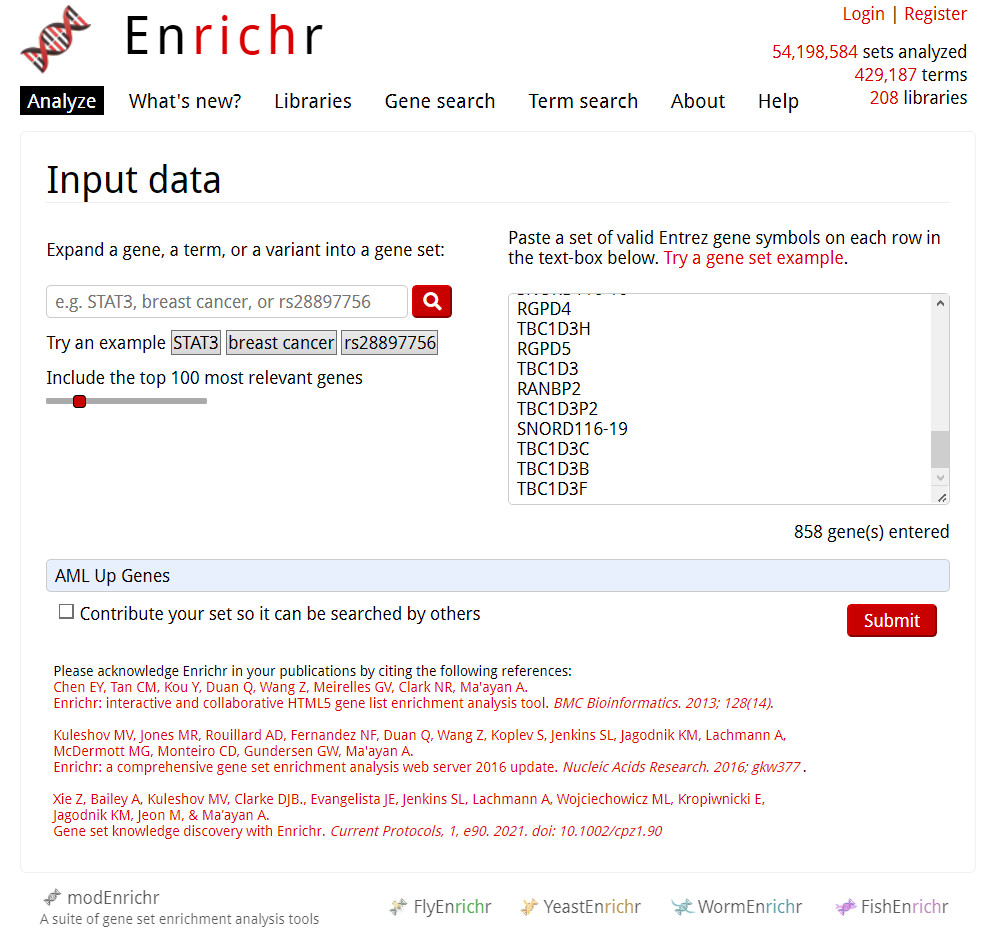
\includegraphics[width=0.5\columnwidth]{figs/enrichr.jpg}
	\caption{وارد کردن داده‌ها برای شروع آنالیز}
	\label{fig:enrichr}
\end{figure}

\subsubsection{انتخاب تمام نمونه‌های سالم}
در بخش \lr{pathways} (شکل \ref{fig:enrichr-pathways}) می‌توان پایگاه‌داده‌های \lr{pathway} مختلف را بررسی کرد.
\begin{figure}[h!]
	\centering
	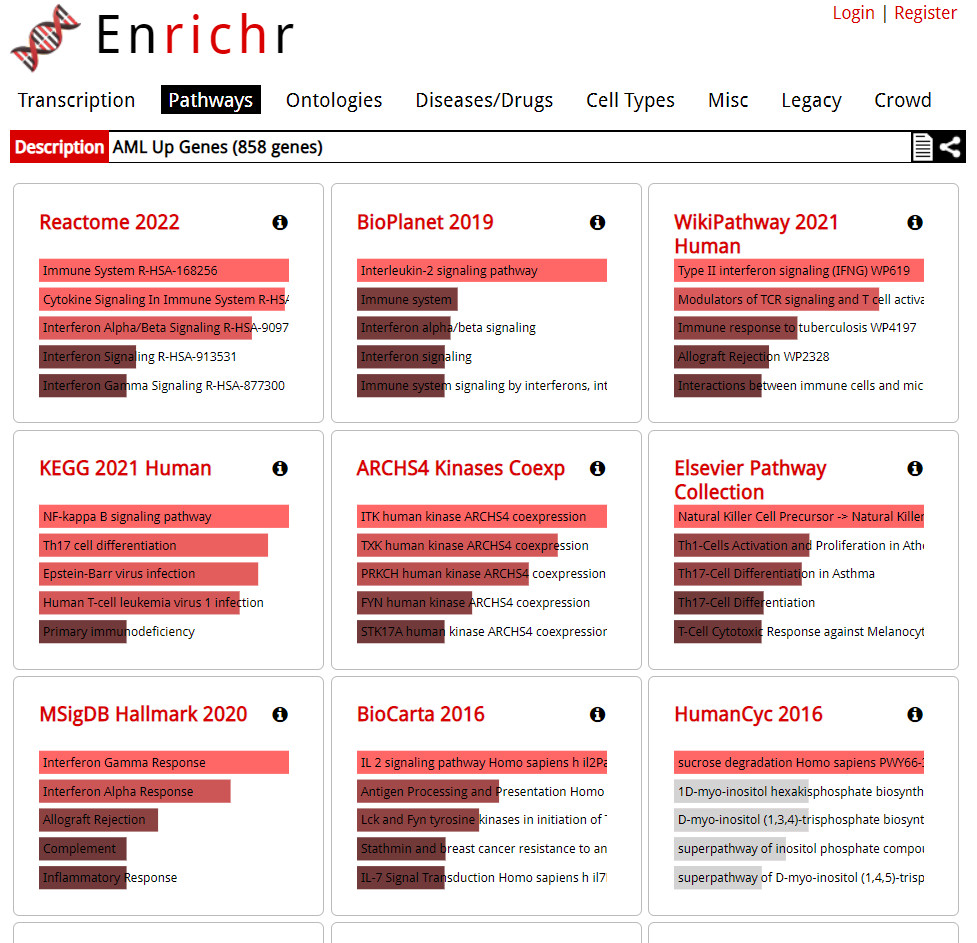
\includegraphics[width=0.5\columnwidth]{figs/enrichr-pathways.jpg}
	\caption{بخش \lr{pathways} در \lr{enrichr} برای ژن‌های بیشتر بیان‌شده و تمام نمونه‌ها}
	\label{fig:enrichr-pathways}
\end{figure}

به‌عنوان مثال در پایگاه‌داده \lr{Reactome 2022} (شکل \ref{fig:enrichr-pathways-reactome}) تعداد زیادی از ژن‌هایی که میزان بیان بیشتری داشتند مربوط به \lr{pathway} سیستم ایمنی \LTRfootnote{\lr{Immune System}} هستند.
\begin{figure}[h!]
	\begin{subfigure}{.59\columnwidth}
		\centering
		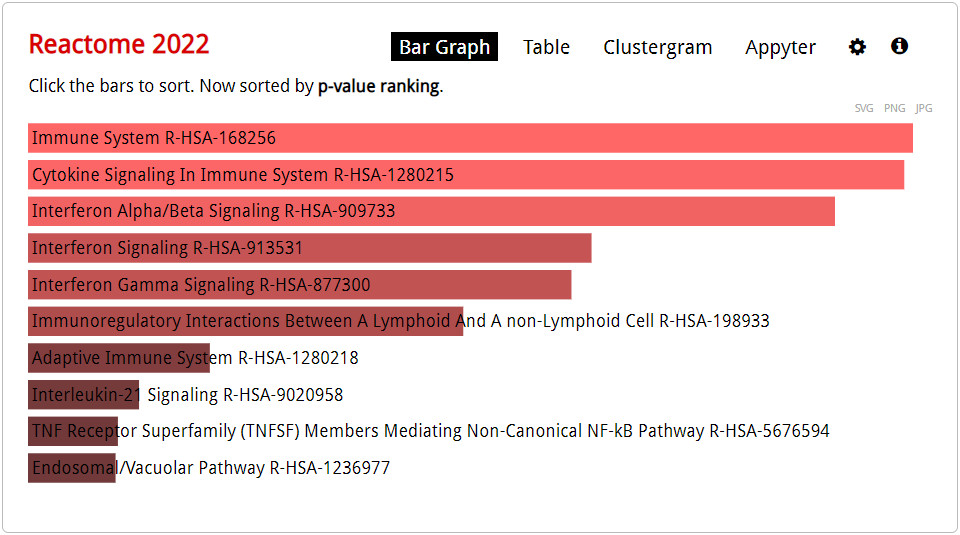
\includegraphics[width=\columnwidth]{figs/enrichr-pathways-reactome.jpg}
	\end{subfigure}
	\begin{subfigure}{.41\columnwidth}
		\centering
		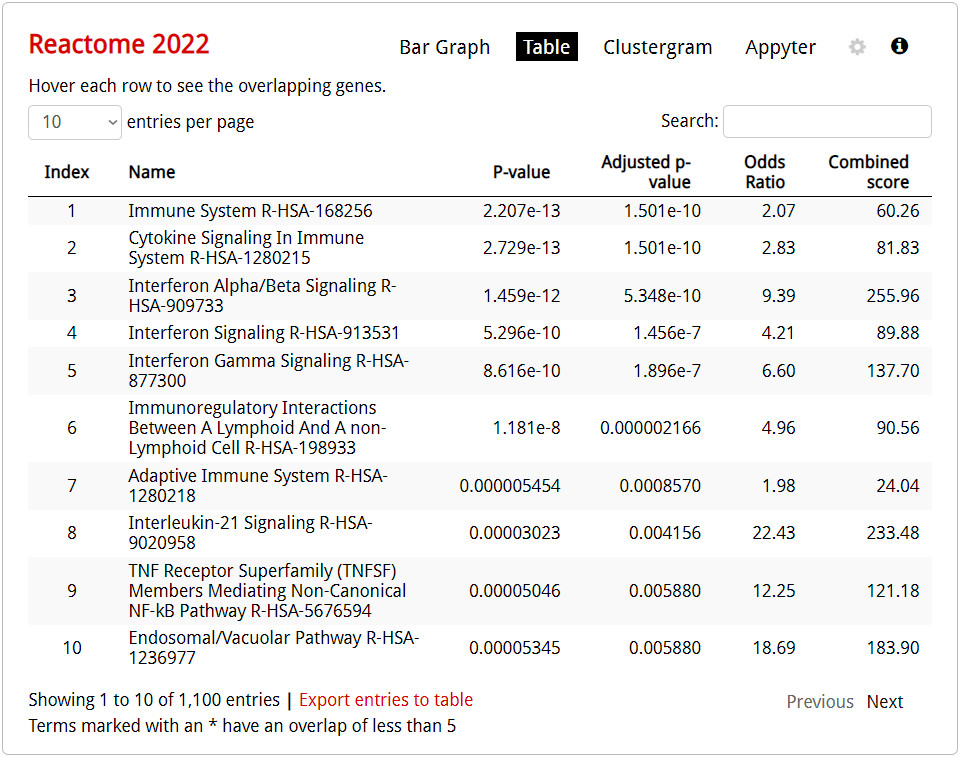
\includegraphics[width=\columnwidth]{figs/enrichr-pathways-reactome-tab.jpg}
	\end{subfigure}
	\caption{\lr{pathway}های پایگاه‌داده \lr{Reactome}}
	\label{fig:enrichr-pathways-reactome}
\end{figure}

و همچنین پایگاه‌داده \lr{KEGG 2021} در شکل \ref{fig:enrichr-pathways-kegg} نمایش داده شده است.
\begin{figure}[h!]
	\begin{subfigure}{.53\columnwidth}
		\centering
		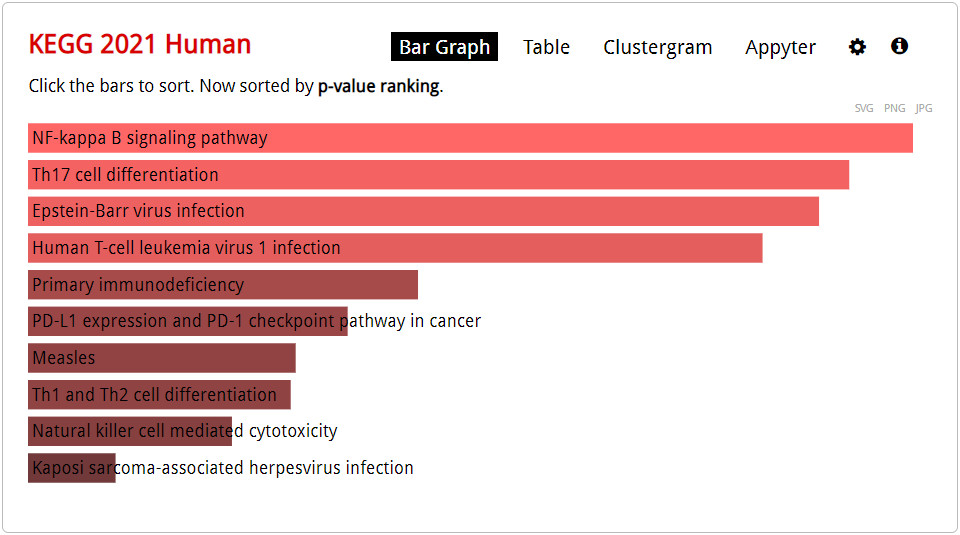
\includegraphics[width=\columnwidth]{figs/enrichr-pathways-kegg.jpg}
	\end{subfigure}
	\begin{subfigure}{.47\columnwidth}
		\centering
		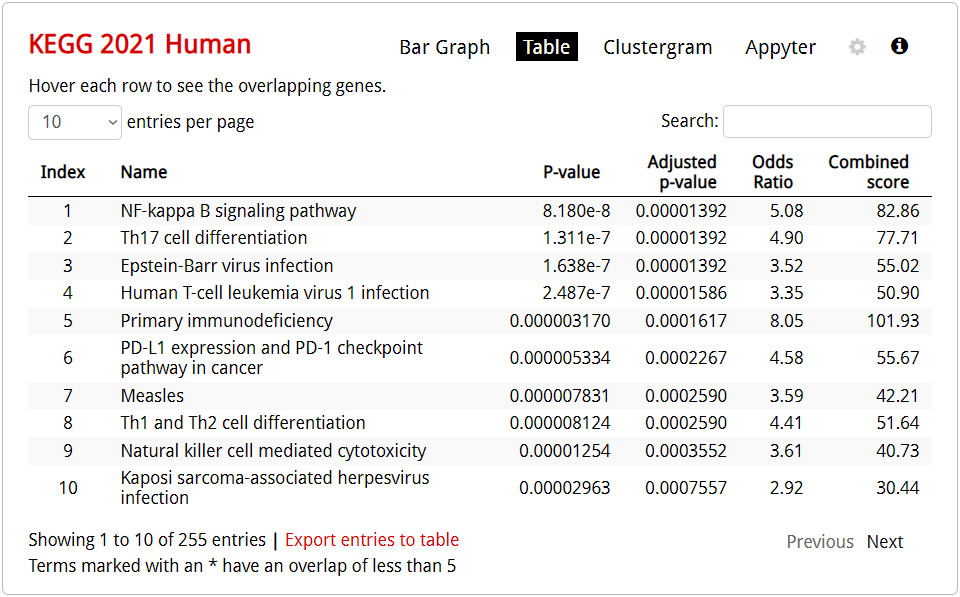
\includegraphics[width=\columnwidth]{figs/enrichr-pathways-kegg-tab.jpg}
	\end{subfigure}
	\caption{\lr{pathway}های پایگاه‌داده \lr{KEGG}}
	\label{fig:enrichr-pathways-kegg}
\end{figure}

در بخش \lr{ontologies} می‌توان \lr{biological processes} (شکل \ref{fig:enrichr-ontology-bp}) و \lr{cellular components} (شکل \ref{fig:enrichr-ontology-cc}) و \lr{molecular functions} (شکل \ref{fig:enrichr-ontology-mf}) را بررسی کرد (شکل \ref{fig:enrichr-ontology}).
\begin{figure}[h!]
	\centering
	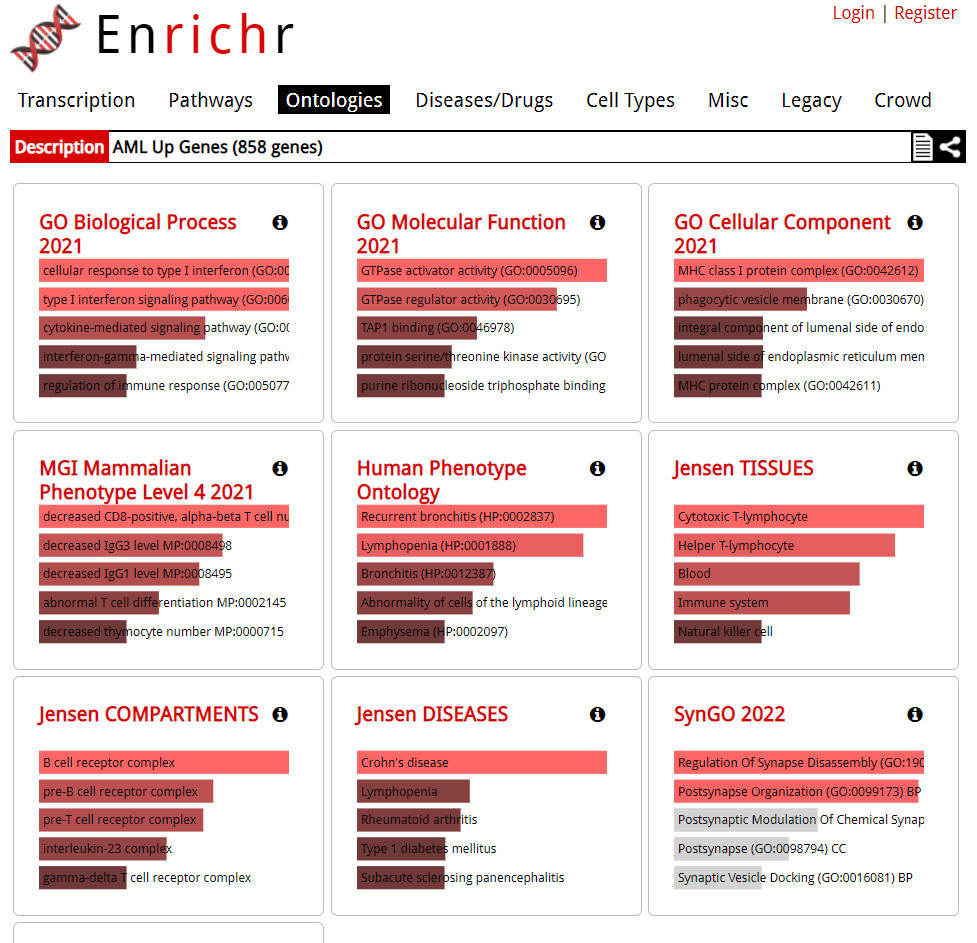
\includegraphics[width=0.5\columnwidth]{figs/enrichr-ontologies.jpg}
	\caption{بخش \lr{ontologies} در \lr{enrichr} برای ژن‌های بیشتر بیان‌شده و تمام نمونه‌ها}
	\label{fig:enrichr-ontology}
\end{figure}

\begin{figure}[h!]
	\centering
	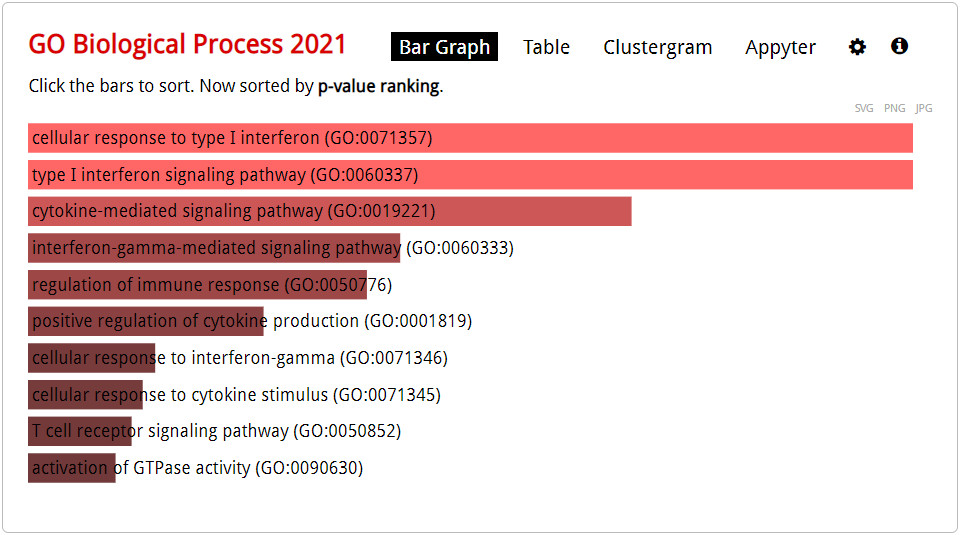
\includegraphics[width=0.5\columnwidth]{figs/enrichr-ontologies-bp.jpg}
	\caption{\lr{biological processes} در بخش \lr{ontologies}}
	\label{fig:enrichr-ontology-bp}
\end{figure}

\begin{figure}[h!]
	\centering
	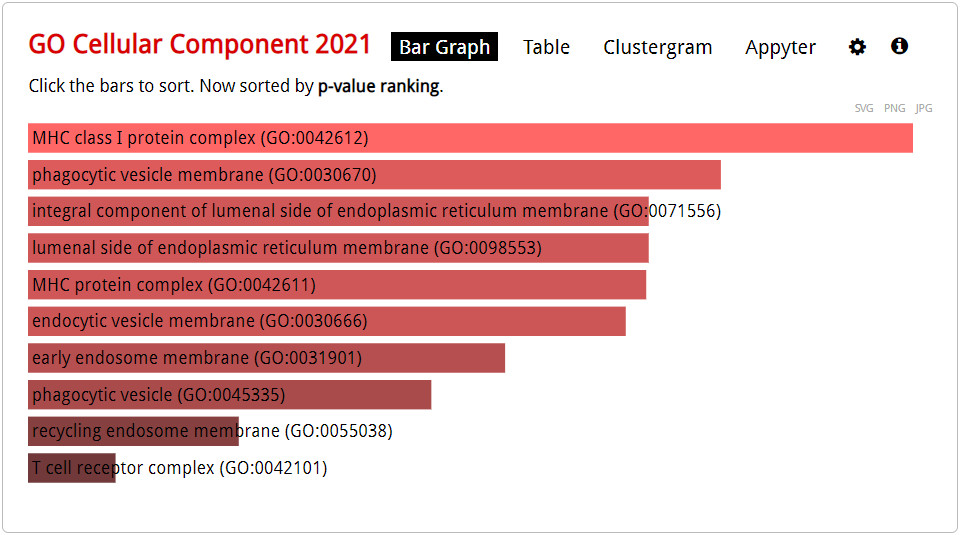
\includegraphics[width=0.5\columnwidth]{figs/enrichr-ontologies-cc.jpg}
	\caption{\lr{cellular components} در بخش \lr{ontologies}}
	\label{fig:enrichr-ontology-cc}
\end{figure}

\begin{figure}[h!]
	\centering
	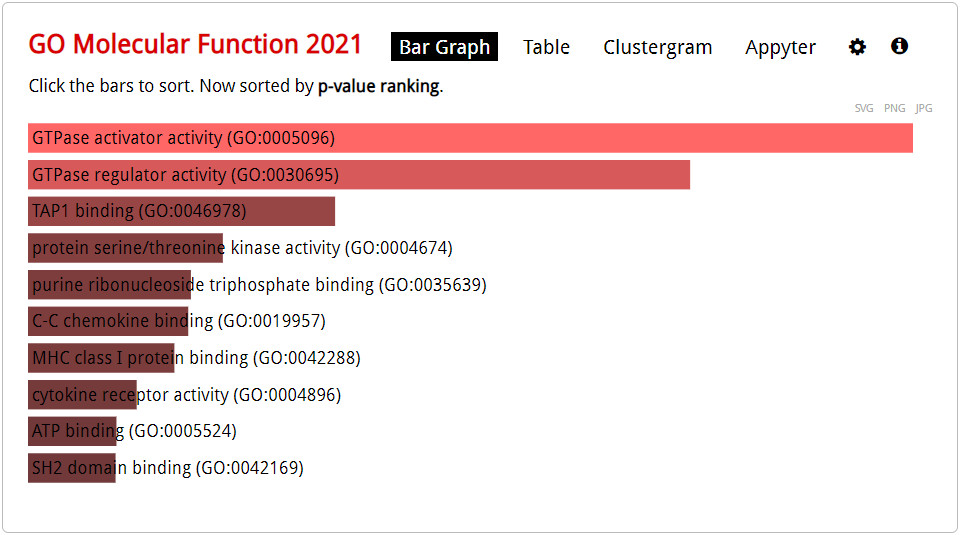
\includegraphics[width=0.5\columnwidth]{figs/enrichr-ontologies-mf.jpg}
	\caption{\lr{molecular functions} در بخش \lr{ontologies}}
	\label{fig:enrichr-ontology-mf}
\end{figure}

\subsubsection{انتخاب نمونه‌های سالم با بیشترین هم‌بستگی}
دوباره با رفتن به بخش \lr{pathways} (شکل \ref{fig:enrichr-pathways-2}) می‌توان پایگاه‌داده‌های \lr{pathway} مختلف را این‌بار برای نمونه‌های جدید بررسی کرد.
\begin{figure}[h!]
	\centering
	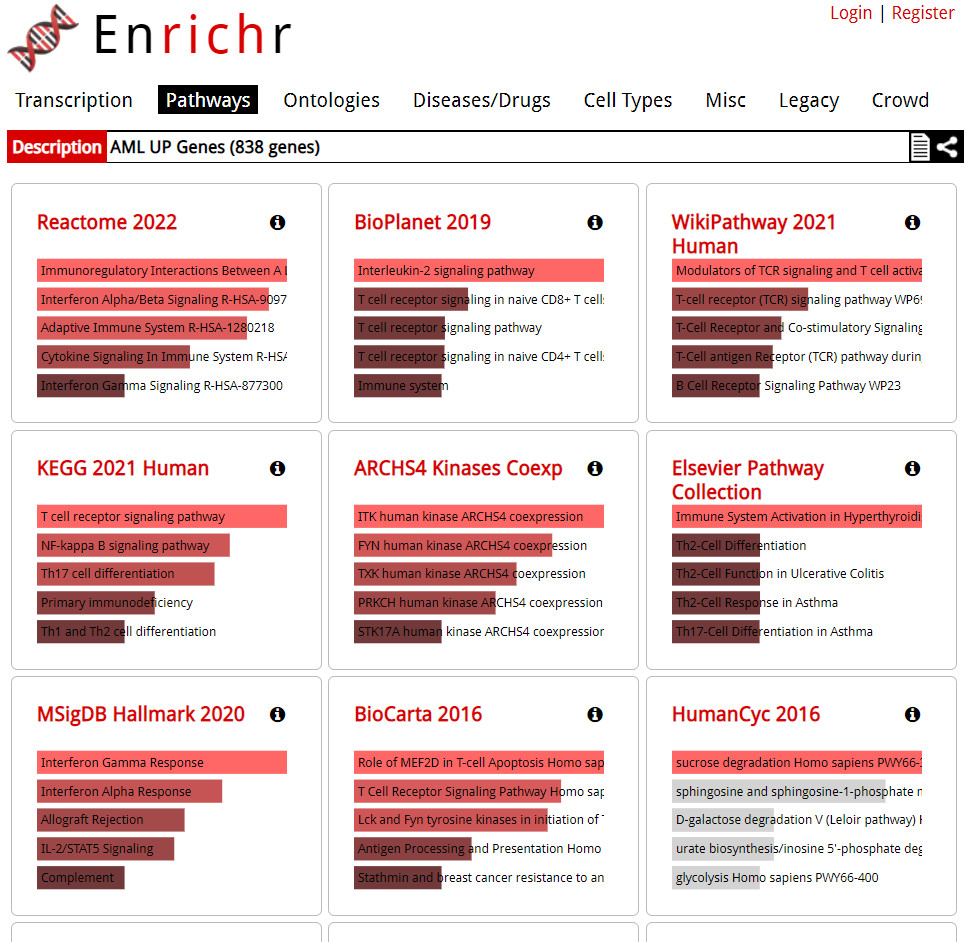
\includegraphics[width=0.5\columnwidth]{figs/enrichr-pathways-2.jpg}
	\caption{بخش \lr{pathways} در \lr{enrichr} برای ژن‌های بیشتر بیان‌شده و نمونه‌های با هم‌بستگی بیشتر}
	\label{fig:enrichr-pathways-2}
\end{figure}

پایگاه‌داده \lr{Reactome 2022} و همچنین پایگاه‌داده \lr{KEGG 2021} در شکل \ref{fig:enrichr-pathways-reactome-kegg} نمایش داده شده است.

\begin{figure}[h!]
	\begin{subfigure}{.5\columnwidth}
		\centering
		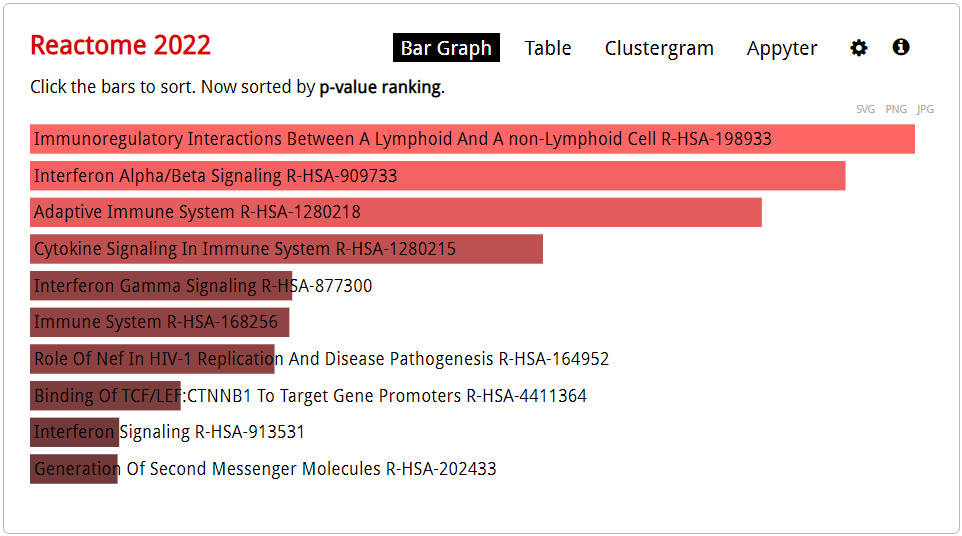
\includegraphics[width=\columnwidth]{figs/enrichr-pathways-reactome-2.jpg}
	\end{subfigure}
	\begin{subfigure}{.5\columnwidth}
		\centering
		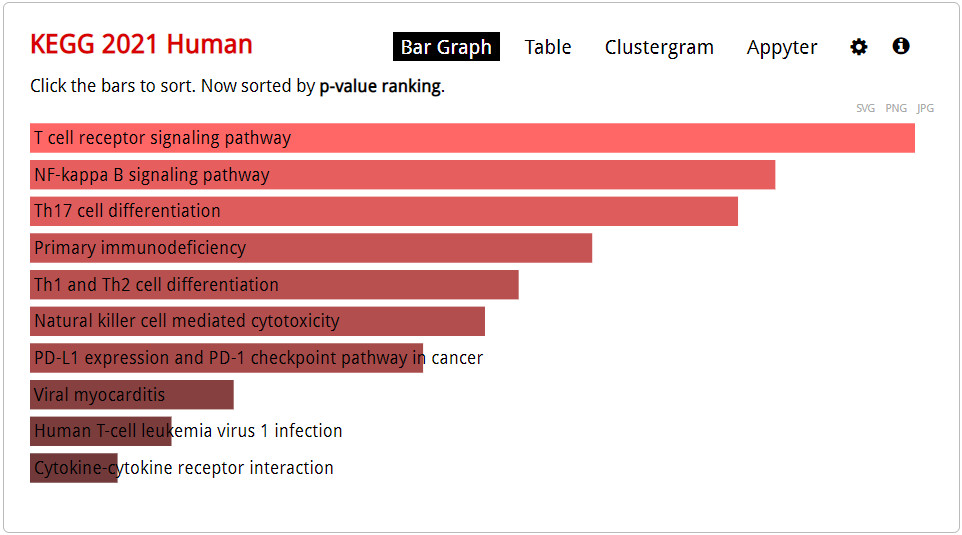
\includegraphics[width=\columnwidth]{figs/enrichr-pathways-kegg-2.jpg}
	\end{subfigure}
	\caption{\lr{pathway}های پایگاه‌داده \lr{Reactome} و \lr{KEGG}}
	\label{fig:enrichr-pathways-reactome-kegg}
\end{figure}

در بخش \lr{ontologies} می‌توان \lr{biological processes} و \lr{cellular components} و \lr{molecular functions} را بررسی کرد (شکل \ref{fig:enrichr-ontology-2}).
\begin{figure}[h!]
	\centering
	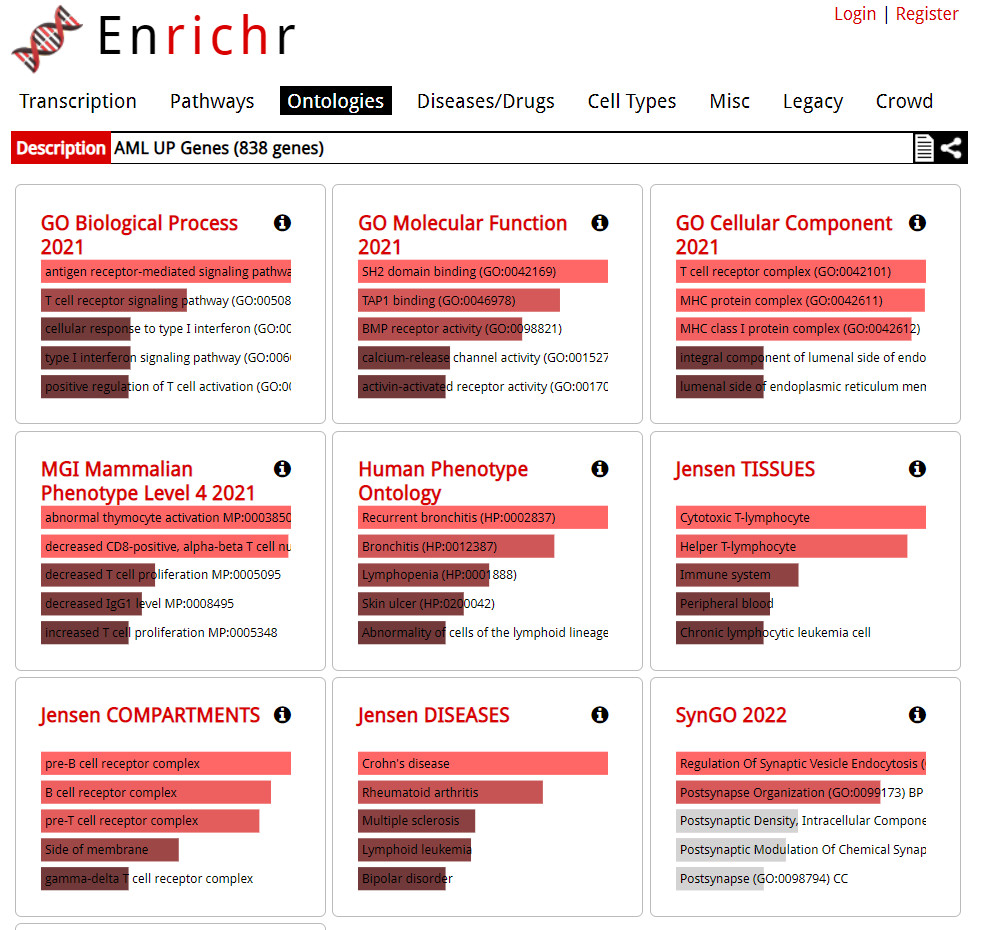
\includegraphics[width=0.5\columnwidth]{figs/enrichr-ontologies-2.jpg}
	\caption{بخش \lr{ontologies} در \lr{enrichr} برای ژن‌های بیشتر بیان‌شده و نمونه‌های با هم‌بستگی بیشتر}
	\label{fig:enrichr-ontology-2}
\end{figure}

\subsection{ژن‌هایی که کمتر بیان شده‌اند}
حالا لیست ژن‌های کمتر بیان‌شده را بررسی می‌کنیم.

\subsubsection{انتخاب تمام نمونه‌های سالم}
در بخش \lr{pathways} (شکل \ref{fig:enrichr-pathways-d}) می‌توان پایگاه‌داده‌های \lr{pathway} مختلف را بررسی کرد.
\begin{figure}[h!]
	\centering
	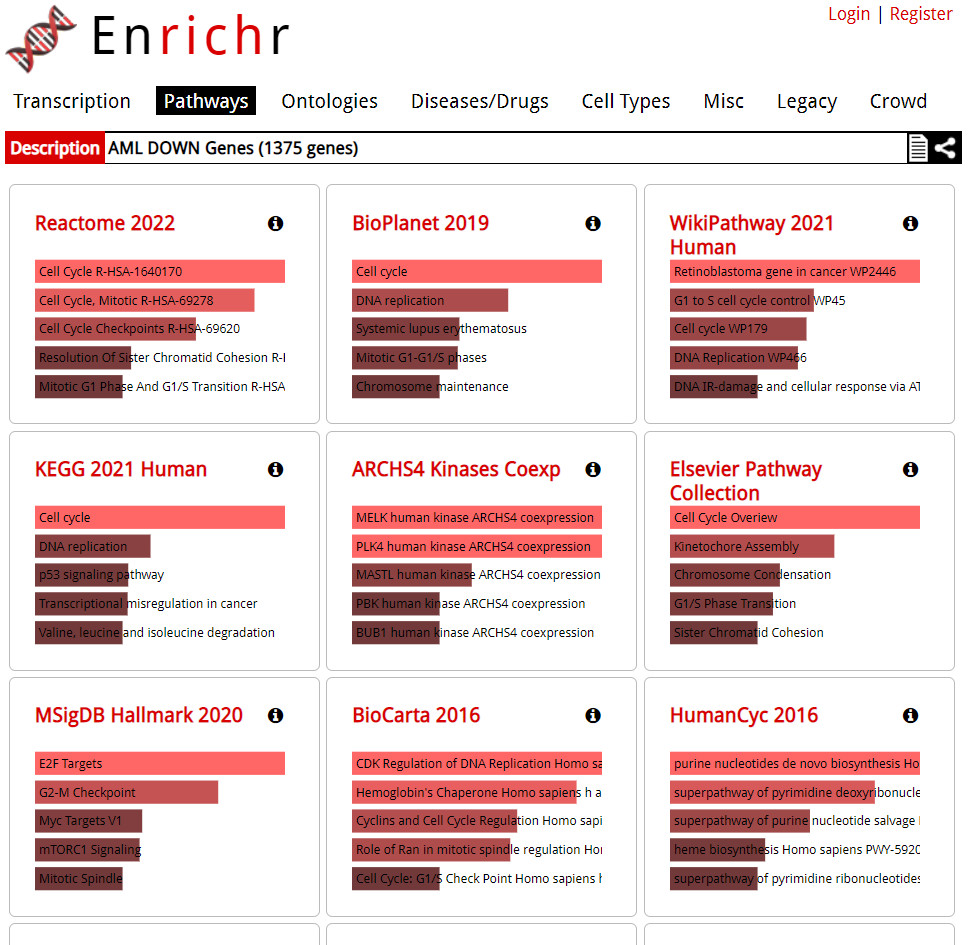
\includegraphics[width=0.5\columnwidth]{figs/enrichr-pathways-d.jpg}
	\caption{بخش \lr{pathways} در \lr{enrichr} برای ژن‌های کمتر بیان‌شده و تمام نمونه‌ها}
	\label{fig:enrichr-pathways-d}
\end{figure}

در بخش \lr{ontologies} می‌توان \lr{biological processes} و \lr{cellular components} و \lr{molecular functions} را بررسی کرد (شکل \ref{fig:enrichr-ontology-d}).
\begin{figure}[h!]
	\centering
	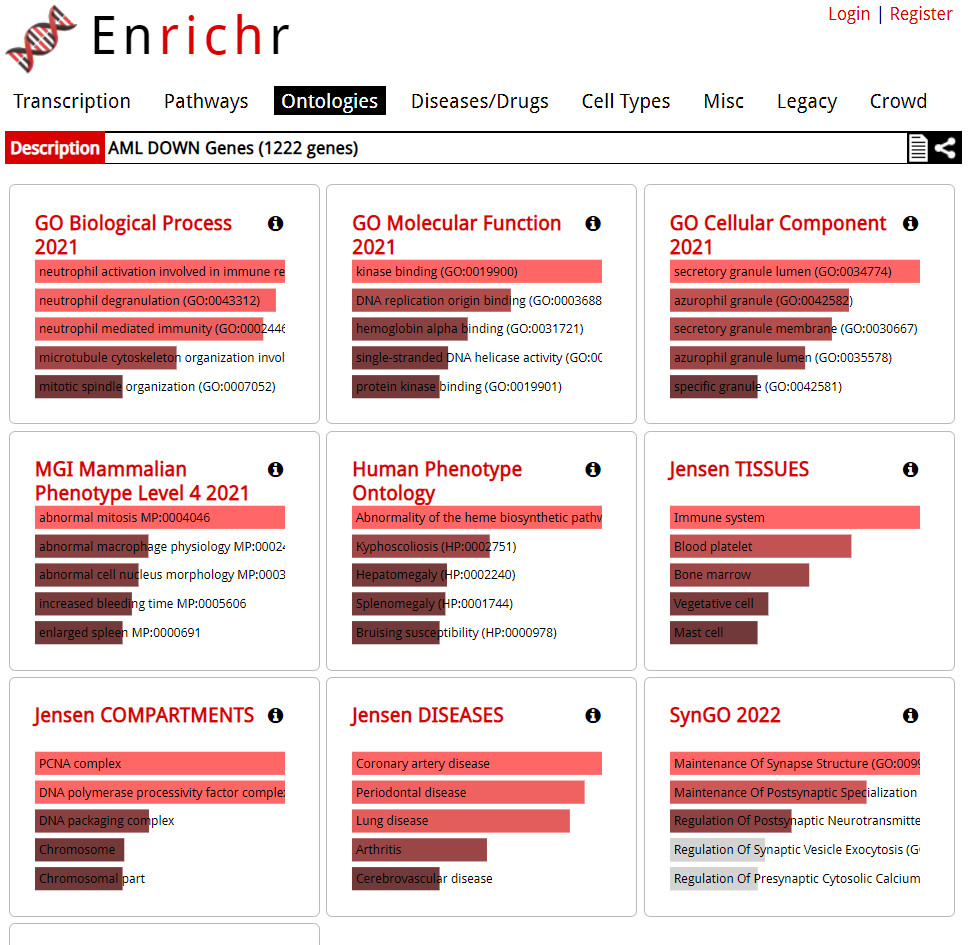
\includegraphics[width=0.5\columnwidth]{figs/enrichr-ontologies-d-2.jpg}
	\caption{بخش \lr{ontologies} در \lr{enrichr} برای ژن‌های کمتر بیان‌شده و تمام نمونه‌ها}
	\label{fig:enrichr-ontology-d}
\end{figure}

\subsubsection{انتخاب نمونه‌های سالم با بیشترین هم‌بستگی}
دوباره با رفتن به بخش \lr{pathways} (شکل \ref{fig:enrichr-pathways-d-2}) می‌توان پایگاه‌داده‌های \lr{pathway} مختلف را این‌بار برای نمونه‌های جدید بررسی کرد.
\begin{figure}[h!]
	\centering
	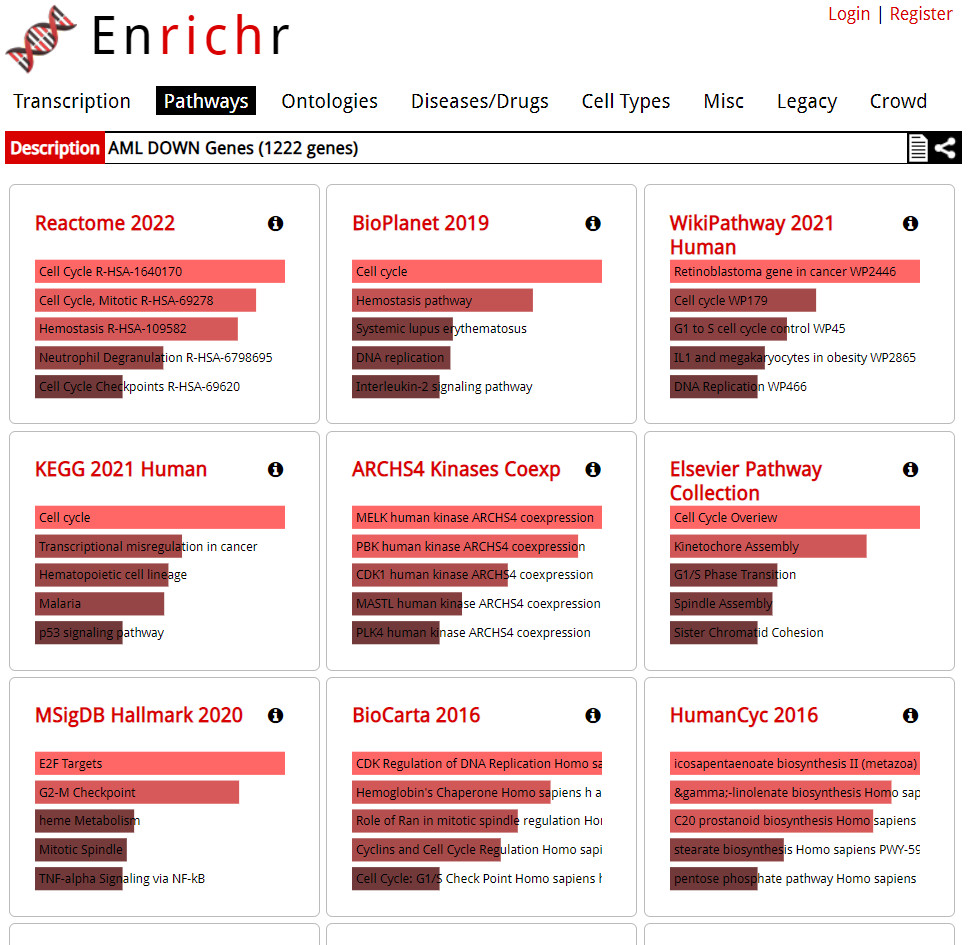
\includegraphics[width=0.5\columnwidth]{figs/enrichr-pathways-d-2.jpg}
	\caption{بخش \lr{pathways} در \lr{enrichr} برای ژن‌های کمتر بیان‌شده و نمونه‌های با هم‌بستگی بیشتر}
	\label{fig:enrichr-pathways-d-2}
\end{figure}

در بخش \lr{ontologies} می‌توان \lr{biological processes} و \lr{cellular components} و \lr{molecular functions} را بررسی کرد (شکل \ref{fig:enrichr-ontology-d-2}).
\begin{figure}[h!]
	\centering
	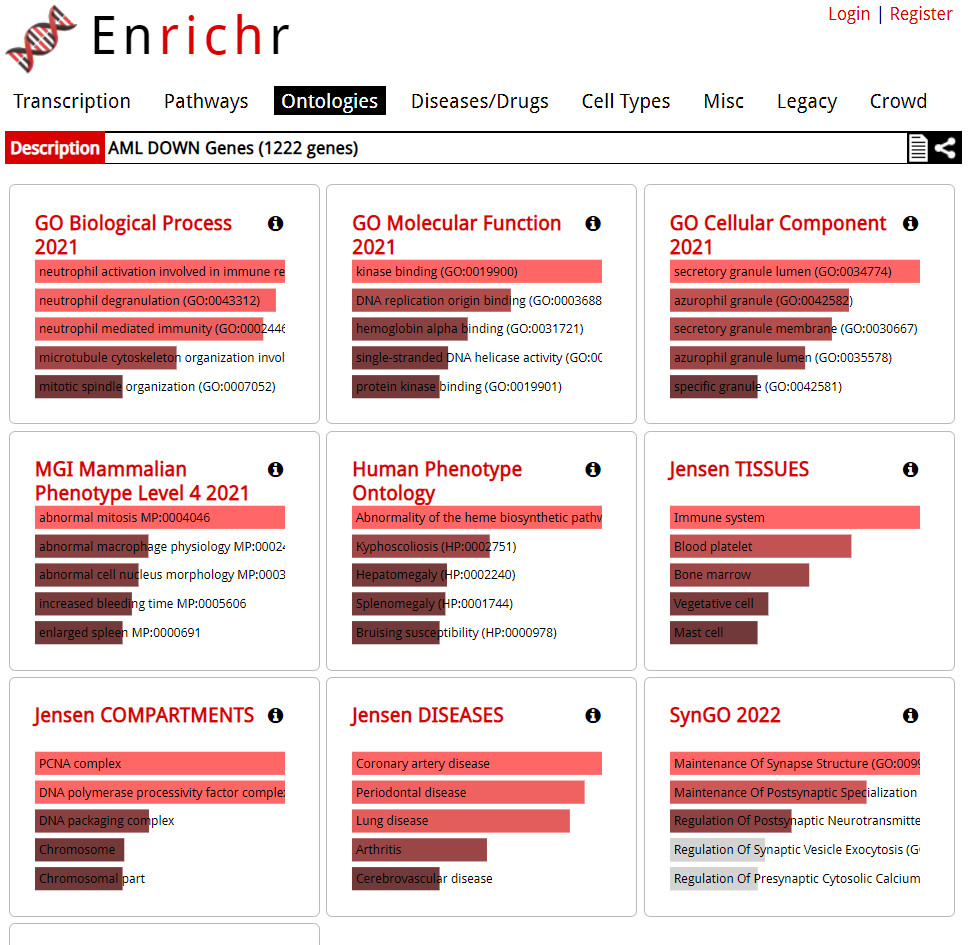
\includegraphics[width=0.5\columnwidth]{figs/enrichr-ontologies-d-2.jpg}
	\caption{بخش \lr{ontologies} در \lr{enrichr} برای ژن‌های کمتر بیان‌شده و نمونه‌های با هم‌بستگی بیشتر}
	\label{fig:enrichr-ontology-d-2}
\end{figure}

\section{جست‌و‌جو در مقالات}
\subsection*{الف)}
پس
\subsection*{ب)}
پس

\clearpage

\begin{thebibliography}{99}
	\begin{latin}
%		\bibitem{nature-microarray}
%		Nature Defenition Microarray (2014), Nature Education, \url{https://www.nature.com/scitable/definition/microarray-202}
		
%		\bibitem{lamport94
%		Leslie Lamport (1994) \emph{\LaTeX: a document preparation system}, Addison
%		Wesley, Massachusetts, 2nd ed.
	\end{latin}
\end{thebibliography}



\end{document}
